%! TEX program = xelatex

\documentclass[a4paper, punct, space=auto, UTF8, fontset = windowsnew, AutoFakeBold]{ctexart}

\usepackage{szutils}%在这里放置需要的宏包,并设置部分所需内容

\begin{document}

\pagestyle{empty}%不要页眉页脚
%封面与诚信声明

%\centerline{\kaishu\zihao{-0}{深圳大学}}
\begin{figure}[htbp]
	\begin{center}
		
\includegraphics[width=2.7in]{szu}
	\end{center}
\end{figure}


\centerline{\heiti\zihao{1}{本\ 科\  毕\  业\  论\  文\  (设计)}}

\vskip 3.5cm



\begin{flushleft}
	\zihao{3}
	\hspace{3cm}{\heiti{题目:}}      
	{\kaishu\underline{\quad\hspace{1.0cm}\textbf{司法语料标注系统}\hspace{2.0cm}}}               \\
	\vspace{10bp}
	
	\hspace{3cm}{\heiti{姓名:}}      
	{\kaishu\underline{\hspace{2.8cm}\textbf{叶志杰}\hspace{3.5cm}}}              \\
	\vspace{10bp}
	
	\hspace{3cm}{\heiti{专业:}}     
	{\kaishu\underline{\hspace{1.5cm}\textbf{计算机科学与技术}\hspace{2cm}}}            \\
	\vspace{10bp}
	
	\hspace{3cm}{\heiti{学院:}}      {\kaishu\underline{\hspace{1.5cm}\textbf{计算机与软件学院}\hspace{2cm}}}               \\
	\vspace{10bp}
	
	\hspace{3cm}{\heiti{学号:}}      {\kaishu\underline{\hspace{2.4cm}\textbf{2015300091}\hspace{2.4cm}}}                   \\
	\vspace{10bp}
	
	\hspace{3cm}{\heiti{指导教师:}} 
	{\kaishu\underline{\hspace{1.8cm}\textbf{李俊杰}\hspace{3.4cm}} }                         \\
	\vspace{10bp}
	
	\hspace{3cm}{\heiti{职称:}}      
	{\kaishu\underline{\hspace{3cm}\textbf{副教授}\hspace{3.3cm}} }                         \\
	
\end{flushleft}

\vskip 4cm

\centerline{\zihao{3} 2019 年 \ \ \ \  月\ \ \ \ \ 日}
\newpage

\centerline{\heiti\zihao{-2}{深圳大学本科毕业论文(设计)诚信声明}}


\vskip 3cm 


\begin{spacing}{2.0}
	\zihao{4}
本人郑重声明:所呈交的毕业论文(设计),题目《司法语料标注系统》是本人在指导教师的指导下,独立进行研究工作所取得的成果。对本文的研究做出重要贡献的个人和集体,均已在文中以明确方式注明。除此之外,本论文不包含任何其他个人或集体已经发表或撰写过的作品成果。本人完全意识到本声明的法律结果。

\vskip 3cm

{\flushright{
		毕业论文(设计)作者签名:\hspace{2.2cm}
		
		

		\hspace{7.5cm}{日期:\hspace{2cm}年 \hspace{.5cm}月\hspace{.5cm}日}\hspace{4cm} 
	}}
\end{spacing}





\zihao{-4}

\tableofcontents %生成目录


\thispagestyle{empty}%页脚不要页码

%“目录”两个字的样式与section的样式一致,默认居中,故将设置section标题居左放置在生成目录后 
\ctexset{
    section={format={\Large\bfseries}},  %section标题居左
}

%%%%正文开始,页脚有页码
\cfoot{\zihao{-5}第 \ \thepage \ 页 \ 共 \ \pageref{lastpage} 页}%%%%lastpage为末页标签
%正文
\zihao{5}
\pagenumbering{arabic}%页码使用阿拉伯数字
\setcounter{page}{0}  %重新设置页码计数
\pagestyle{fancy}

\newpage


\centerline{\fangsong\bf\zihao{-2}{司法语料标注系统}}
\addcontentsline{toc}{section}{摘要(关键词)}%加入目录


\vskip 1cm

\begin{center}
	\kaishu
	\hspace{2cm}计算机与软件学院计算机科学与技术专业 \quad 叶志杰
	\vspace{5bp}
	\newline
	学号:2015300091
\end{center}

\vskip 10bp

{
\kaishu	
\hspace{5bp}{\zihao{-4}\textbf{【摘要】}} 
在律师和法官的日常工作中,筛选判决书和从判决书里提取出关键纠纷占据了很大的人力成本。本文针对这一痛点,提出了自动提取法律判决书中关键纠纷的方法。训练集为一批法律判决书。首先对获取到的训练集进行中文预处理,包括中文切词、去除停用词、word2vec词向量化、构建司法领域词典等操作。然后对从原文档词向量化出来的词向量,使用Kmeans算法进行多次迭代聚类,并通过评估簇心平均距离进行快速筛选。筛选得到一批簇后,对这批簇使用svm算法进行训练,训练出来的模型已经具有能分辨法律判决书中关键纠纷的能力了。实验结果表明,此方法效果良好,能有效地从判决书中提取出关键纠纷,大幅度减少人工提取法律文书中的关键纠纷的成本。

\vskip 10bp

\hspace{5bp} {\zihao{-4}\textbf{【 关键词】}} 
法律文书; KMeans; 文本标注; word2vec; SVM; 关键因子
}
\section{引言}

\subsection{研究背景及意义}
随着社会的进步与发展,以及信息逐渐趋向透明、公开化,越来越多案件的审判过程与结果暴露在公众的视野下,接受着公众的监督。然而,在同一件案子下,不同的法官可能会得出不同的审判结果,这是因为每个人都有自己的评判标准。在此情形下,让案件得到公正的审判、减少个人尺度标准差异带来的影响,变得尤为重要。通过本论文提出的方法,能够训练出一个模型,该模型可以从当前判决书中提取出关键因子,再通过多项关键因子推荐相似的已判决过的案件,这些案件给法官作为一个参考,以减少个人因素带来的影响,除此之外,此技术还能帮助减轻法官,律师的工作量,让他们能把精力更多地投入到案子。这能带来一个更公正的审判结果,从而引导一个和谐的社会舆论氛围。

随着最高人民法院对审判流程信息、裁判文书信息、执行信息全面公开的推进,中国裁判文书网在此背景下诞生,作为全国法院统一的裁判文书公开平台,裁判文书生效后七日内都将被传送至中国裁判文书网公布累计只2017年的统计,库内判决书已达3247万篇\cite{WEB:judgement},这繁杂的信息中,有很多信息对律师法官,乃至人民群众来说,都有很高的参考价值,如何利用好这么大的数据,就要使用到自然语言处理技术(NLP)

律师与法官在接受到一个案子的时候,首先要做的就是从案件中提取关键点。关键点就是这个案子的争议焦点、历史判决、双方诉称辩称、引用的法律发条等等。然后,根据这些关键点,去裁判文书网中搜索类似的案件作为参考。但是这样检索存在两个问题,一是关键点通常都是一句陈述句,并且在不同案件下,同一个意思往往有好几种表达方法,这类关键句在裁判文书网中往往检索不到想要的结果。二是检索到的结果都是弱相关的,仍然需要用户进一步自行筛选。这样的流程得出来的结果是低效,精准度差的。

得益于数据挖掘中的文本挖掘的发展,以上痛点均可通过自然语言处理技术来解决。首先从裁判文书网获取若干判决书作为训练姐,再对训练集进行中文预处理,以句来切分,对所有的句子使用Kmeans聚类算法来聚类,从聚类结果中挑选出符合关键因子特征的簇,作为一类关键因子。通过反复的迭代与挑选,可以选出足够数量的簇,足以覆盖绝大多数的关键点。再用这些簇来训练出一个分类模型,即可得出一个能从新的判决书中分类出关键句子的模型。在这个过程中,聚类的质量直接影响了分类模型的精准度。本人在此项目中主要从事聚类相关工作,因此本文主是要围绕聚类算法来展开研究,对比多种聚类算法的质量。

\subsection{国内外研究现状}
虽然很早之前,就有人开始研究自然语言处理,但真正提出用计算机来处理自然语言,是在1950年。当时,艾伦图灵提出了一个标准,意为能通过”图灵测试“\cite{WEB:turing_test}标准的程序可以被判断为是智能的。概念提出之后一直到1980年代,人们研发的NLP系统都是基于规则的,由复杂的规则堆砌而成,那时候的人们调侃这种系统为“积木系统”,对于超过规则之外的输入,这种系统只能给出机械式的,无关痛痒的回答。1980年之后,人们把机器学习引入了NLP来提升它的准确性和稳定性。除此之,NLP还因为两个革新效果大幅度提升,一是运算能力稳定增加(硬件的性能和价格遵守摩尔定律),二是转换-生成文法方法的乔姆斯基语言学理论不再是NLP的主要方法\cite{WEB:turing_test}。从此之后,各领域的NLP技术稳步发展,逐渐走向成熟。

近期,已经有人开始把深度学习的技巧也引入NLP,在自然语言处理方面取得了巨大的成就,如Yonghui Wu等人发表的Exploring the Limits of Language Modeling\cite{DBLP:journals/corr/JozefowiczVSSW16}。但本文只研究基于无监督学习的聚类算法。

作为NLP的重要分析手段,聚类分析,是当下的一个热门研究对象。在聚类分析的发展进程中,产生了大量的聚类算法,主流的为以下几种:中心聚类、层次聚类、密度聚类、谱聚类等。

聚类算法的目的,通俗地来讲,是将具有共性的样本归类为统一类别,再将少有甚至没有共性的样本归类为不同类别。这里的共性通常是通过度量样本之间的距离来求得的,对距离的定义有很多种,我们需要结合样本的特点来具体分析。\cite{ZW:cluster_alg_study_compare}

总之,聚类算法最终是要得到一批符合以下亮点特征的簇的集合:一是每个簇(又称为类簇)内的距离相对紧密,二是不同簇的簇间距离相对较大。

\subsection{研究目的与主要工作}
由于我们获取的数据未经过标注,无法进行分类模型训练,故我们需要把这些数据搭上类标签。一般的做法是通过人工标注来标记分类关键因子。但人工标注的时间和经济成本耗费较大,如何高效、低成本地标注数据呢?本文从聚类的角度出发,通过聚类算法,把一堆原始数据聚成若干个簇后再筛选、评估,最终得到覆盖较为全面的类簇集合。

本文主要研究的聚类算法是KMeans\cite{Macqueen67somemethods}算法和GSDMM\cite{Yin:2014}算法

\subsubsection{KMeans算法}

KMeans算法的主要思想是寻找每个簇的中心,再把与中心具有共性的点归类的该中心所代表的类簇中。KMeans算法是迭代执行的,需要给出有一个参数K,K为预估的类簇的数量。初始的时候,会随机生产K个中心点,在KMeans的每轮迭代中,都会更新K个中心点的位置,重复迭代,直到K个中心点的位置不再变化,此时可以判断为收敛了,所得的K个点的集合,经过筛选之后,即可选为最终的类簇。用KMeans算法的好处是收敛速度比较快,因为其计算比较简单,是通过不断计算距离来迭代更新的,这个距离一般是欧式距离。

\subsubsection{GSDMM算法}
GSDMM算法是一个基于Dirichlet多项式混合模型的算法,发表自清华大学信息科学与技术国家实验室的尹建华和尹建勇\cite{Yin:2014},其算法给出了一个通俗易懂的例子来理解这个算法:一位教授正在教一个电影课。在课程开始时,学生被随机分配到K个桌子。在课程开始前,学生们列出一个他们最喜欢的电影的表单。教授则反复阅读每一位学生的表单。每次叫到一位学生的时候,这位学生会被分配到至少满足以下一个条件的新桌子去:
\begin{enumerate}
	\item 新桌子的学生比当前学生所在的桌子的学生多
	\item 新桌子的学生的电影清单都是相似的
\end{enumerate}
通过不断地迭代,预期所有的学生都会被分配到“最优”的桌子去。GSDMM算法的好处是无需指定K值,该算法会自动调整K值,并且根据作者的测试结果,GSDMM的耗时比KMeans少了4/5。

\subsection{本章小结}

本章主要介绍了相关需求背景和聚类算法的发展历史,对KMeans算法和GSDMM算法进行了粗浅的初步解释,在第三章中我会更加细致地解释这两种算法。

\section{文本预处理}
在自然语言处理中,数据源处理的好坏直接影响到跑出来的模型的效果,可见,文本预处理在自然语言处理中是尤为重要的一环。对于不同语言的文本,预处理的过程是不一样的。对于英文,由于词与词之间已经用空格分隔开了,要做的只是把英文单词的时态和单复数等问题解决就行。

但是对于中文文本来说,由于词与词之间不存在间隔,无法直接分词,需要借助分词工具。同样,分词的效果好坏直接影响了聚类的效果。本章主要介绍我在中文文本预处理中执行的三大操作:名词归一化替换、中文分词、word2vec词向量化。

\subsection{非专业名词归一化替换}

在一份没有经过任何处理的法律文书中,往往充斥着大量原告被告、地名、金额、日期、数量、时间、期限、法律法条等信息,这类信息若不处理,会导致下一步的中文分词分错,进而使得聚类模型跑偏,结果不准确。
但是这类信息也是有效的,单纯地去掉也会导致关键因子的丢失,故采用替换为统一的名词来处理,比如原告名字统一替换为“原告”,金额数据统一替换为“金额”等等。

本文使用了两种方法来替换原文:一种是基于词典的替换,另一种是基于正则的替换。在网络上可以找到很全的地名字典,故可以直接用地名字典去匹配原文中的地名,然后统一替换成“地址”。

剩下的非专业名词使用正则表达式来进行替换。所用正则表达式如下:
\begin{itemize}
	\item \textbf{大数目金额}:\zihao{-4.5}$(([1-9]\backslash \backslash d*[\backslash \backslash d,,]*\backslash \backslash .?\backslash \backslash d*)|(0\backslash \backslash .[0-9]+))$(元|百万|万元|亿元)

	\item \textbf{原、被告名字}: \zihao{-4.5}$((?<=($原告|被告$)$:$).*?(?=$,$|\/|$。|、))

	\item \textbf{日期}:\zihao{-4.5}$\backslash$d$\{$4$\}$(年)$\backslash$d$\{$1,2$\}$(月)$\backslash$d$\{$1,2$\}$(日)|(?:$\backslash$d$\{$1,2$\}$|[$\backslash$u4e00-$\backslash$u9fa5])(?:个月|个星期|个工作日|日)|$\backslash$d$\{$4$\}$(年)$\backslash$d$\{$1,2$\}$(月)|$\backslash$d$\{$1,2$\}$(月)$\backslash$d$\{$1,2$\}$(日)|$\backslash$d$\{$4$\}$(> >
	年)|$\backslash$d$\{$1,4$\}$(日)

	\item \textbf{利息}: \zihao{-4.5}($\backslash$d*($\backslash$.$\backslash$d*)?(?:$\backslash$\%|%|‰))|(百|千|万)分之[$\backslash$u4e00-$\backslash$u9fa5]$\{$1,2$\}$(点[$\backslash$u4e00-$\backslash$u9fa5])?|($\backslash$d(分))

	\item \textbf{数量}: \zihao{-4.5}((?:$\backslash$d|[$\backslash$u4e00-$\backslash$u9fa5])(?:份|张|次))
	
	\item \textbf{期限}: \zihao{-4.5}(?:$\backslash$d$\{$1,2$\}$|[$\backslash$u4e00-$\backslash$u9fa5])(?:个月|个星期)|[$\backslash$u4e00-$\backslash$u9fa5]月|$\backslash$d$\{$1,3$\}$(天)
\end{itemize}

通过上述正则表达式,匹配替换原词为指定的统一词汇,可以让文本的结构更加清晰,同时又保留了这部分关键词,分词的准确率有了很大的提升。

\subsection{中文分词}
中文分词,是自然语言处理中的最基本的问题,如果中文分词不正确,中文NLP的其他算法也无法进行下去。由于中文的字与词是相连的,没有一个结构化的方法来划分,故需要一些算法来把它们分成独立的词,目前常用的分词方法有五种。

第一种是\textbf{正向最大匹配},最大正向匹配是基于词典的匹配,首先设置一个最长窗口长度。然后从句子左边开始,向右扫描,每次移动一格,若窗口内有词语出现在了词典中,则标记该词语。这种算法能在大多数情况下生效,但是一旦句子里有多义词或未登陆词\footnote{\label{unlogin_word}未登陆词:词典中未录入的词语},那这个算法将无法识别。第二种是\textbf{逆向最大匹配},这种算法原理跟正向最大匹配一样,只是窗口滑动方向是从最右边的词尾开始,滑向词头。第三种是\textbf{双向最大匹配},这个算法同时运用了正向最大匹配和逆向最大匹配,得到两种匹配的结果后对比,若两种分词的结果一样,那就认为是切分成功,采用分词结果。若两种算法的分词结果不一致,则表明出现了歧义现象或者出现了未登录词语。第四种是\textbf{N-gram双向最大匹配}。Ngram算法是基于统计的分词,他是通过计算样本的所有切分方案的概率,选择概率最大的那个。这个模型是基于一个这样的假设,一个句子中,第n个词的出现只与前面n-1个词相关,与其他句子中的词不相关。设$W_i$为句子中每个词的概率,$P \left( T \right)$为当条句子的概率,如公式\ref{ngram_approx}所示,整条句子的概率,约等于这个句子中每个词的概率的乘积。第五种是\textbf{基于隐马尔科夫模型(HMM)的分词},HMM模型主要是解决未登陆词的问题。

\begin{equation}
	\begin{aligned}
		P(T) &= P(W_1W_2W_3…W_n) \\
				&= P(W_1)P(W_2|W_1)P(W_3|W_1W_2)…P(W_n|W_1W_2…W_{n-1}) \\
				&\approx P(W_1)P(W_2|W_1)P(W_3|W_2)…P(W_n|W_{n-1})\\
	\end{aligned}
\label{ngram_approx}
\end{equation}


本文采用的是\textbf{jieba分词}的分词词工具,结巴分词主要是采用
\begin{itemize}
	\item 基于前缀的词典实现的词图扫描,对句子中的汉字的所有成词情况,生成有向无环图 (DAG)
	\item 通过动态规划来查找最大概率路径, 找到基于词频的最大切分组合
	\item 采用了HMM模型,并使用$Viterbi$算法算法优化,解决了未登陆词的问题
\end{itemize}

测试数据表明,jieba分词能正确地切分绝大多的句子,即使句子中有未登陆词,jieba分词也能正确地切分出来,在处理一些极端的情况,如“结婚的和尚未结婚的”这种句子,jieba分词也能正确地切分。


\subsection{Word2Vec词向量化}
经过了jieba分词的处理,我们已经把每个句子转化为词语组成的集合,但是聚类算法主要是通过计算两个向量的距离来判断两个样本的相似度,所以我们光拿词语组成的集合是不够的。还需要把词语转换成向量。

把句子转化为向量的方法大致有两种,1.通过词袋模型转换,2. 通过词向量模型转换


\subsubsection{词袋模型}
词袋模型,顾名思义也就是将所有词语装进一个袋子里,不考虑其词法和语序的问题,即每个词语都是独立的。
词袋模型最常用的方法是One-Hot Encoding,即把数据中所有词语去重后,一一映射到一个大小与去重词语数量相等的数组上,数组的每元素值都只能为0或者1,0表示映射到该下标的词语没有出现,1表示映射到该下标的词语出现了。具体例子如下

\newpage
首先给出两个简单的样本,如下所示: 

\begin{enumerate}
	\item $[$ He, is, a, male $]$
	\item $[$ She, is, a, female $]$
\end{enumerate}

根据上面两个例句,就可以构成一个词袋,袋子中含有的词为He、She、is、a、male、female,假设构建一个数组[He, She, is, a, male, female]来匹配映射,那么上面两句话可以转化成以下两组向量来表示

\begin{enumerate}
	\item $[$ 1, 0, 1, 1, 1, 0 $]$
	\item $[$ 0, 1, 1, 1, 0, 1 $]$
\end{enumerate}
	
这两个词频向量就是基于词袋模型转换出来的向量,可以看出,这样转换的坏处是语境上下文完全丢失了,只保留了单词出现的频率,这是不足以完全展示一个句子的含义。

同时,当你的词袋内的词越多,向量的纬度就会越大。我在一开始做词向量化的时候用的就是词袋模型,导致我的向量的纬度是十几万!这运行起来简直是个灾难,速度非常慢。所以一般我们不用原生的词袋模型来做词向量化。

\subsubsection{词向量模型}

    词向量模型是考虑词语位置关系的一种模型。通过大量语料的训练,将每一个词语映射到高维度(几千、几万维以上)的向量当中,通过求余弦的方式,可以判断两个词语之间的关系,例如例句中的Jane和Bob在词向量模型中,他们的余弦值可能就接近1,因为这两个都是人名,Shenzhen和Bob的余弦值可能就接近0,因为一个是人名一个是地名。

    现在常用word2vec构成词向量模型,它的底层采用基于CBOW和Skip-Gram算法的神经网络模型。

1. CBOW模型

    CBOW模型的训练输入是某一个特征词的上下文相关的词对应的词向量,而输出就是这特定的一个词的词向量。比如上面的第一句话,将上下文大小取值为2,特定的这个词是"go",也就是我们需要的输出词向量,上下文对应的词有4个,前后各2个,这4个词是我们模型的输入。由于CBOW使用的是词袋模型,因此这4个词都是平等的,也就是不考虑他们和我们关注的词之间的距离大小,只要在我们上下文之内即可。

    这样我们这个CBOW的例子里,我们的输入是4个词向量,输出是所有词的softmax概率(训练的目标是期望训练样本特定词对应的softmax概率最大),对应的CBOW神经网络模型输入层有4个神经元,输出层有词汇表大小个神经元。隐藏层的神经元个数我们可以自己指定。通过DNN的反向传播算法,我们可以求出DNN模型的参数,同时得到所有的词对应的词向量。这样当我们有新的需求,要求出某4个词对应的最可能的输出中心词时,我们可以通过一次DNN前向传播算法并通过softmax激活函数找到概率最大的词对应的神经元即可。


\begin{figure}[htbp]
	\centering
	\begin{subfigure}{.5\textwidth}
		\centering
		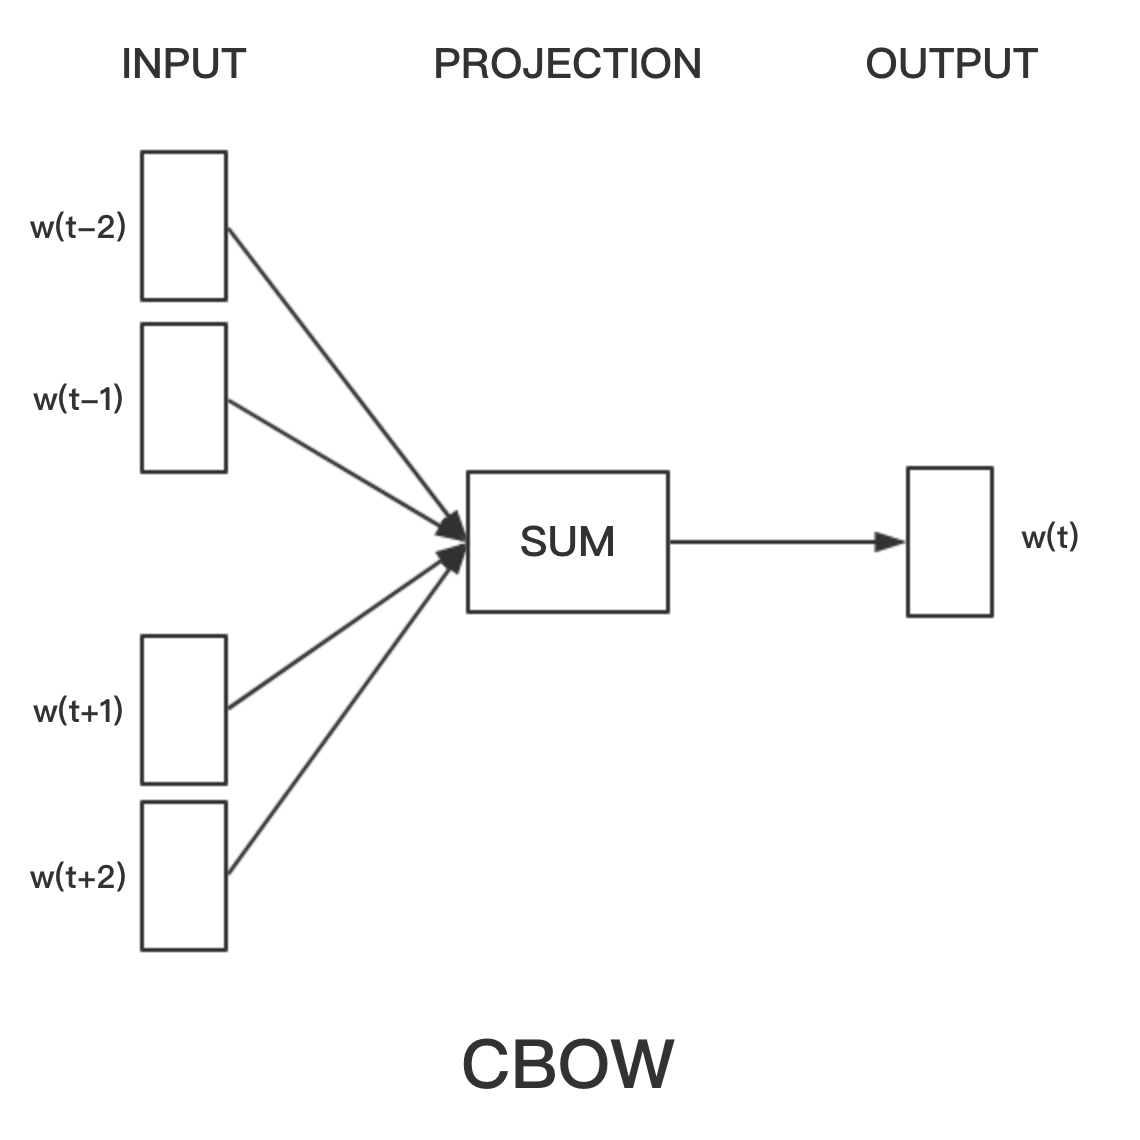
\includegraphics[width=1\linewidth]{cbow.png}
		\caption{CBOW 模型}
		\label{word_vec:cbow}
	\end{subfigure}%
	\begin{subfigure}{.5\textwidth}
		\centering
		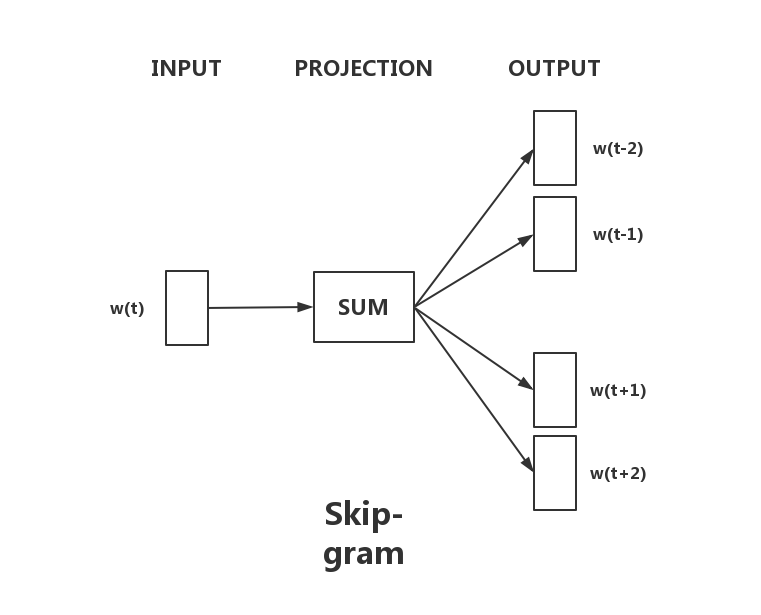
\includegraphics[width=1\linewidth]{Skip-gram.png}
		\caption{Skip-Gram 模型}
		\label{word_vec:skip_gram}
	\end{subfigure}
	\caption{词向量模型}
	\label{word_vec:example}
\end{figure}

2.Skip-Gram模型

    Skip-Gram模型和CBOW的思路是反着来的,即输入是特定的一个词的词向量,而输出是特定词对应的上下文词向量。还是上面的例子,我们的上下文大小取值为2, 特定的这个词"go"是我们的输入,而这4个上下文词是我们的输出。

    这样我们这个Skip-Gram的例子里,我们的输入是特定词, 输出是softmax概率排前4的4个词,对应的Skip-Gram神经网络模型输入层有1个神经元,输出层有词汇表大小个神经元。隐藏层的神经元个数我们可以自己指定。通过DNN的反向传播算法,我们可以求出DNN模型的参数,同时得到所有的词对应的词向量。这样当我们有新的需求,要求出某1个词对应的最可能的4个上下文词时,我们可以通过一次DNN前向传播算法得到概率大小排前4的softmax概率对应的神经元所对应的词即可。

词向量模型突出特点:

    在词向量模型中,词向量与词向量之间有这非常特殊的特性。例如现在存在国王、男生、女人、皇后四个词向量,那么一个完善的词向量模型,就存在“国王-男人+女人=皇后”这样的关系。

\section{算法实现与结果分析}

\label{analize}

第\ref{analize}章将对以上提到的算法和改进进行实证研究,以评估算法的效率和改进方案。\ref{analize_subsection_1}节将介绍实验中使用的数据集、查询参数以及实验平台。4.2节将评估基于密度k-STC查询的改进方案。

\subsection{实验环境}
\label{analize_subsection_1}

本章的数据集来自网站kaggle上188593组餐厅信息,每组信息包括店铺ID,地理位置以及菜单信息。每家餐厅的文字描述长度平均为8个单词。具体来说,我们将18万组数据生成了大小为10k,50k,100k,150k,180k的数据集。利用不同的数据集测试算法性能。在180k的数据集中

在180k的数据集中随机选择一个对象p,利用位置偏离得到一个新的对象,新的对象文本描述保持一致。从对象的文本中随机选取单词作为查询关键字,关键词数量为1,2,3。因为查询集是对象文本的子集,所以不会有查询为空的情况。

实验评估了基本方法(basic)、带权重的IR-树的优化方法(Adv)。表\ref{args_scale}显示了实验中使用的参数值,其中粗体值是默认值。所有算法均采用Java语言实现,实验采用Intel(R) Core(TM) i5-4590 CPU @ 3.30GHz,内存8GB。所有的数据结构都保存在内存中。实验记录k-STC查询所需的平均运行时间。

\begin{table}[h!]
  \begin{center}
    \renewcommand\arraystretch{1.5}
    \begin{tabular}{|c|c|c|}
      \hline
      描述 & 参数 & 取值 \\
      \hline
      请求集群数 & $\left|q.\psi \right|$ & $1,2,3$ \\
      \hline
      \multirow{2}*{密度约束} & \varepsilon & $1,2,10,20,50$  \\
      \cline{2-3}
      ~ & $minpts$ & 1$0, 20, 50, 100$ \\
      \hline
      平均参数 &  $\alpha$ & $0.1, 0.3, 0.5, 0.7, 0.9$ \\
      \hline
      数据集大小 &$ \left| D \right|$ & $10k, 50k, 100k, 150k, 180k$ \\
      \hline
    \end{tabular}
    \caption{参数取值}
    \label{args_scale}
  \end{center}
\end{table}
\section{引言}

\subsection{研究背景及意义}

互联网的出现和普及给用户带来了大量的信息, 满足了用户在信息时代对各种信息的需求, 但随着Internet的迅速发展而带来的网络上信息量的巨幅增长, 使得用户在面对大量信息时无法快速从中获得对自己真正有用的那部分信息。换言之, 在这种情况下人们对信息的使用效率反而降低了, 这就是所谓的信息过载(information overload)问题. 的确如此, 面对信息的汪洋大海, 人们往往感到无所适从, 信息过载已经成为一个不容忽视的问题.

目前, 应对信息过载的办法之一便是以搜索引擎为代表的信息检索系统, 比如国外的Google\footnote{\url{https://www.google.com/}}、国内的Baidu\footnote{\url{https://www.baidu.com/}}等, 它们在帮助用户从巨大的网络资源中获取信息方面发挥着极其重要的作用. 但对于使用搜索引擎的用户而言, 在使用同一个关键字搜索信息时, 在一段时间内所得到的结果都是相同的. 另一方面来看,信息及其传播是多样化的, 而用户对信息的需求是多元化和个性化的, 那么通过以搜索引擎为代表的信息检索系统获得的结果显然不能满足用户的个性化需求, 它们仍然无法很好地解决信息过载问题.

面对信息过载, 另外一个非常有潜力的办法是个性化的推荐系统, 它是根据用户的信息需求、兴趣等, 将用户所感兴趣的信息、产品、服务等推荐给用户的个性化信息推荐系统. 和搜索引擎相比, 推荐系统通过研究用户的历史行为与兴趣偏好, 进行个性化考量, 由系统发现用户的兴趣点, 从而引导用户发现自己的信息需求. 一个优秀的推荐系统不仅能为用户提供个性化的服务, 还能和用户之间建立密切关系, 让用户对其推荐产生依赖. 个性化推荐系统现已广泛应用于很多领域, 其中最典型并具有良好的发展和应用前景的领域就是电子商务领域. 目前,几乎所有大型的电子商务系统,如 Amazon, eBay, 京东, 当当网上书店等, 都不同程度地使用了各种形式的推荐系统。同时学术界对推荐系统的研究热度一直很高, 逐步形成了一个独立的研究领域.

Internet为人们提供了极其丰富的信息资源,在这些海量、异构的Web信息资源中蕴含着具有巨大潜在价值的知识。根据用户访问的历史记录以及各种服务或商品之间的相关信息可以构建用户的兴趣模型,从而凭借该用户的兴趣模型对繁杂的信息进行过滤, 然后向用户推荐其可能感兴趣的服务或商品。事实上, 推荐系统已经成为目前解决信息过载最有效的工具之一。




\subsection{本文主要工作}

本文从推荐系统的概述展开, 讨论了在推荐系统的学习算法中随机梯度下降方式中采用均匀采样策略而导致收敛缓慢的一些原因, 并通过融合内容信息改进了均匀采样策略--适应性采样策略, 然后将适应性采样策略放入已有的推荐算法框架中, 加快原有推荐算法的学习。




\subsection{论文组织结构}

 本论文共分为七章,内容如下: 

 第一章为引言, 主要介绍了本论文的研究背景、意义, 主要工作及论文的组织结构.
 
 第二章为推荐系统概览,并分类介绍了包括了基于内容、基于系统过滤与混合型推荐算法的一些典型的推荐学习算法。
 
 第三章为预备工作,首先简要回顾了Bayesian Personalized Ranking(BPR)推荐算法, 并对其局限性进行了一些探讨。
 
 第四章为适应性采样策略,主要研究了通过融合内容信息提出了适应性采样策略改进已有的均匀采样策略。
 
 第五章为整体的算法框架, 将适应性采样策略融入已有的BPR推荐模型。
 
 第六章为实验论证,主要内容为在适应性采样策略下的推荐算法的实验表现。
 
 第七章为结论与展望,首先简要总结了本文的一些工作,并对接下来进一步的研究工作做了展望。

\include{data/chapter05}
\include{data/chapter06}
\include{data/chapter07}


%参考文献
\kaishu
\bibliographystyle{plain}
\addcontentsline{toc}{section}{参考文献} %向目录中添加条目,以章/section的名义
\bibliography{ref/szuthesis.bib}


%致谢与英文摘要
\fangsong
\newpage

\section*{\centerline{\heiti\zihao{-4}{致谢}}}
\addcontentsline{toc}{section}{致谢}

首先衷心地感谢***老师。在我大学生涯里,给予了很多指导与帮助。本次毕业设计,从选题到论文撰写,给予我很多宝贵的意见。***渊博的学识、严谨的治学态度及认真负责的工作态度都使我受到鼓舞和熏陶。在此向***老师表示崇高的敬意和衷心的感谢。

\vspace{5bp}
感谢研究生刘联东师兄。从毕业设计到毕业论文的撰写,刘联东师兄都给了我很大的帮助,在平时的讨论中给我提出了许多宝贵的意见和建议。他认真负责、热衷钻研的工作学习态度都使我受到很大的激励。在此,向刘联东师兄表示衷心的感谢。

\vspace{5bp}
感谢四年以来老师们的辛勤授课,丰富了我们的知识,拓宽了我们的视野,提高了我们发现问题、解决问题的能力,使我的思想产生了质的飞跃。

\vspace{5bp}
感谢开源社区,提供了很多开放源码与类库,为我提供了庞大的优秀代码资源,使我在程序开发过程中得到很多启发。

\vspace{5bp}
感谢自己熬过了那段难捱的日子。在如今看来似曾是做了诸多无用功, 不过幸而没有因为短时的平庸迷茫而消磨掉满心的戾气. 

\vspace{5bp}
感谢一直关心我、支持我的父母和朋友们。
\newpage

\centerline{\fangsong\bf\zihao{-2}{Research on Content-Aware Collaborative Filtering }}

\addcontentsline{toc}{section}{Abstract(Key words)}

\vskip 20bp

\hspace{4bp} {\zihao{-4}\textbf{【 Abstract】}} 
Pairwise learning algorithms are a vital technique
for personalized ranking with implicit feedback. They usually
assume that each user is more interested in items which have
been selected by the user than remaining ones. This pairwise
assumption usually derives massive training pairs. To deal with
such large-scale training data, the learning algorithms are usually
based on stochastic gradient descent with uniformly drawn pairs.
However, the uniformly sampling strategy often results in slow
convergence. In this paper, we first uncover the reasons of
slow convergence. Then, we associate contents of entities with
characteristics of dataset to develop an adaptive item sampler
for drawing informative training data. In this end, to devise a
robust personalized ranking method, we accordingly embed our
sampler into Bayesian Personalized Ranking (BPR) framework,
and further propose a Content-aware and Adaptive Bayesian
Personalized Ranking (CA-BPR) method, which can model both
contents and implicit feedbacks in a unified learning process. The
experimental results show that our adaptive item sampler can indeed improve recommendation performance.

\vskip 10bp

\hspace{5bp}{\zihao{-4}\textbf{【 Keywords】}}
Recommendation System; Collaborative Filtering; Adaptive Sampling


\vskip 20bp

\begin{flushright}
    \kaishu 指导教师:\ 潘微科 \hspace{3cm}{ }
\end{flushright}

\label{lastpage}%%%%显示总页数

\end{document}
